%alpha-persian-p.userguide
%by: shapour madadpour
%E-mail: madad_sh@yahoo.com
\documentclass{article}
\usepackage[top=4cm,left=3cm,right=3cm,bottom=2.5cm]{geometry}
\usepackage{xcolor}
\usepackage{float}
\parindent0pt
\usepackage[pagebackref=true,colorlinks,linkcolor=blue,citecolor=green!80!black]{hyperref}
\usepackage{amssymb}
\usepackage{amsmath}
\usepackage{verbatim}
\usepackage{fancyvrb}
\usepackage{xcolor}
\usepackage{ragged2e}
\newcommand*\justifyv{%
\fontdimen2\font=0.4em
\fontdimen3\font=0.2em
\fontdimen4\font=0.1em
\fontdimen7\font=0.1em
\hyphenchar\font=`\-
}
\usepackage{fancyhdr}
%\usepackage{url}
\usepackage[compress]{cite} 
%باید دوبار خروجی بگیرید.
%\usepackage[numbers,sort&compress]{natbib}
\usepackage{graphicx}
\usepackage{xepersian}
\settextfont[Scale=1.2]{Yas}
\newcommand{\PRL}[1]{\RL{\Parsifont #1}}
\DefineVerbatimEnvironment{rtlverbatim}{Verbatim}{commandchars=+\[\]}
\newfontfamily\Parsifont[Script=Arabic]{XB Niloofar}
\newcommand{\prl}[1]{\RL{\Parsifont #1}}
\newcommand{\pdflatex}{P\!\!\reflectbox{\raisebox{-1mm}{{\small D}}}F\LaTeX}
\pagestyle{fancy}
\fancyhf{}
\rhead[OR]{\thepage}
\lhead[EL]{\leftmark}
\renewcommand{\headrulewidth}{1pt}
\renewcommand{\footrulewidth}{1pt}
\fancyfoot[C]{{\rl{\color{green!50!black}تهیه‌ کننده: شاپور مددپور}}}
\title{\textbf{
	سبک آلفاپرشین; سبکی برای ایجاد مراجع فارسی و انگلیسی}}
\author{\LARGE{\textbf{نویسنده و نگه‌دارنده‌ی بسته‌: شاپور مددپور}}
\\[1cm]
\LARGE{\textbf{
کارشناس ارشد توپولوژی}}
\\[1cm]
\LARGE{\textbf{
دبیر ریاضی، دبیرستان‌های اهواز}}
}
\begin{document}
\maketitle
\clearpage
\baselineskip=1cm
\tableofcontents\clearpage
\baselineskip=.5cm
\paragraph{\color{red!50!black}سبک ایجاد مراجع، 
\lr{alpha-persian.bst}~  نسخه: 3.1}
\paragraph{\color{red!50!black}19 اسفند 1397}
\paragraph{\color{red!50!black}
نویسنده و نگه‌دارنده‌ی بسته‌: شاپور مددپور}
\paragraph{\color{red!50!black}
ایمیل:
\lr{madad\_sh@yahoo.com}}\hfill

\vspace*{2cm}
سبک آلفاپرشین در اسفندماه  1397 توسط اینجانب ایجاد و در آدرس
زیر از 
\lr{CTAN}
(شبکه‌ی جامع بایگانی تک) و مخزن تکلایو قرار گرفت.
\href{https://ctan.org/tex-archive/biblio/bibtex/contrib/alpha-persian}{https://ctan.org/tex-archive/biblio/bibtex/contrib/alpha-persian}\\[.6cm]
در تصویر زیر نیز می‌توانید محل ثبت و مشخصات آن را در 
\lr{CTAN}
ببینید.
\begin{figure}[H]
\centering
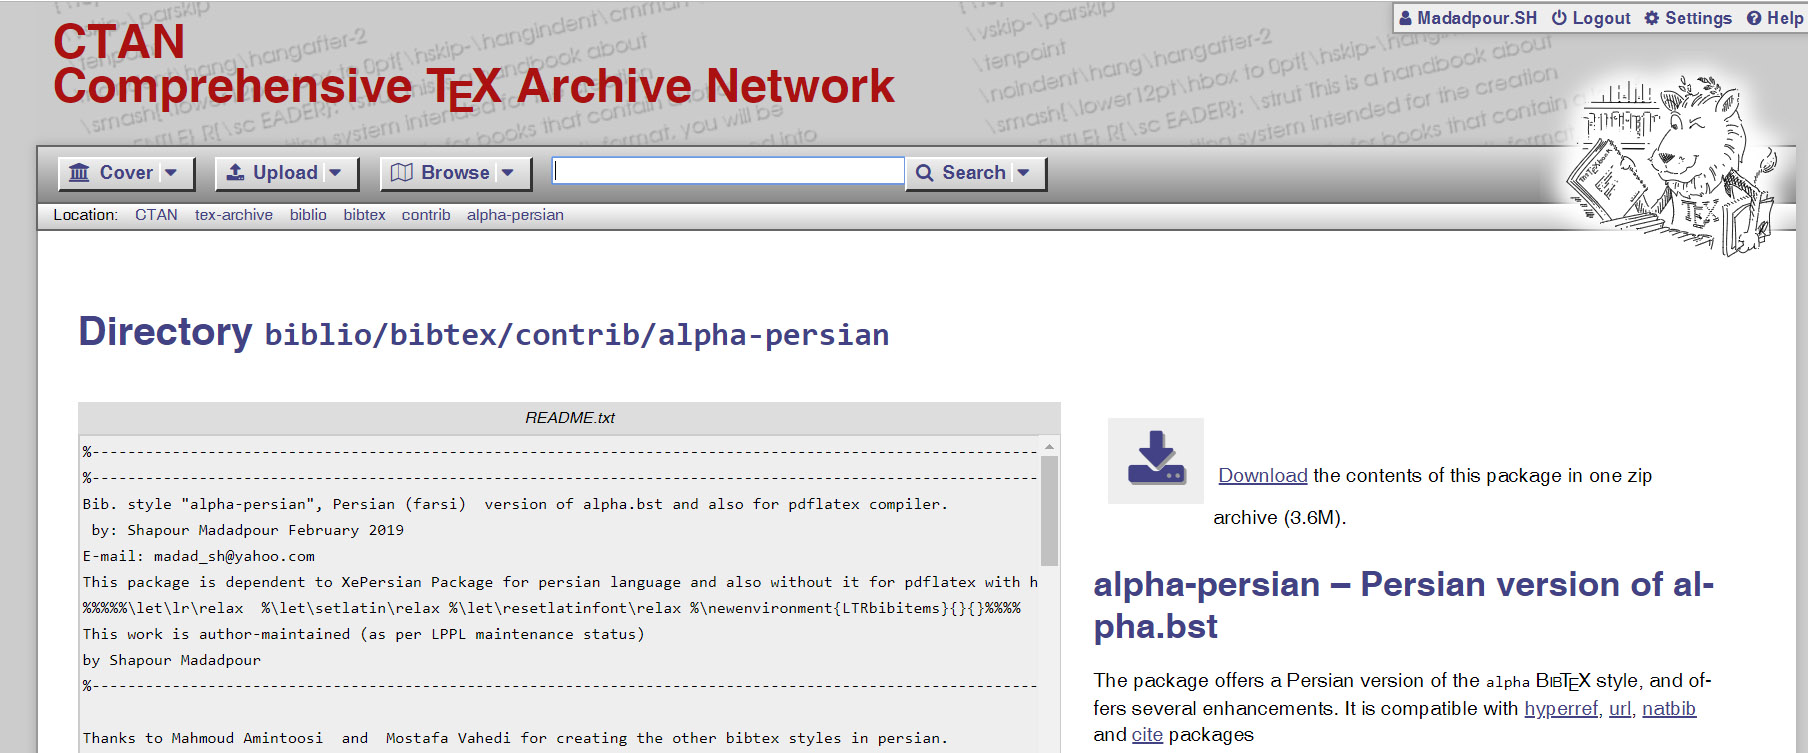
\includegraphics[width=\textwidth,height=7cm]{image/sh18}
\end{figure}\vspace*{-.87cm}
\begin{figure}[H]
\centering
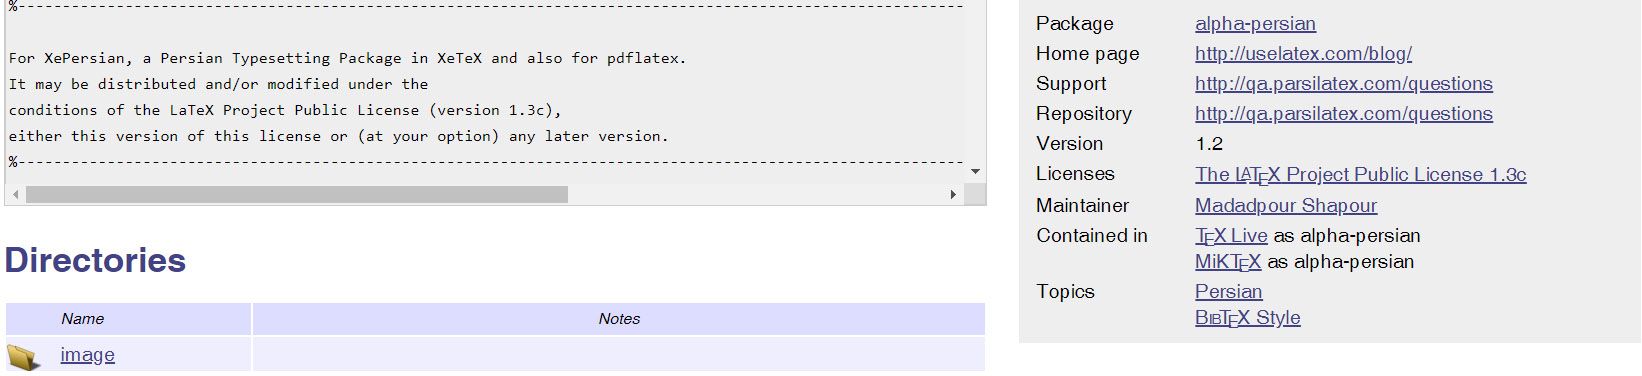
\includegraphics[width=\textwidth,height=4cm]{image/sh20}
 \end{figure}
\begin{figure}[H]
\centering
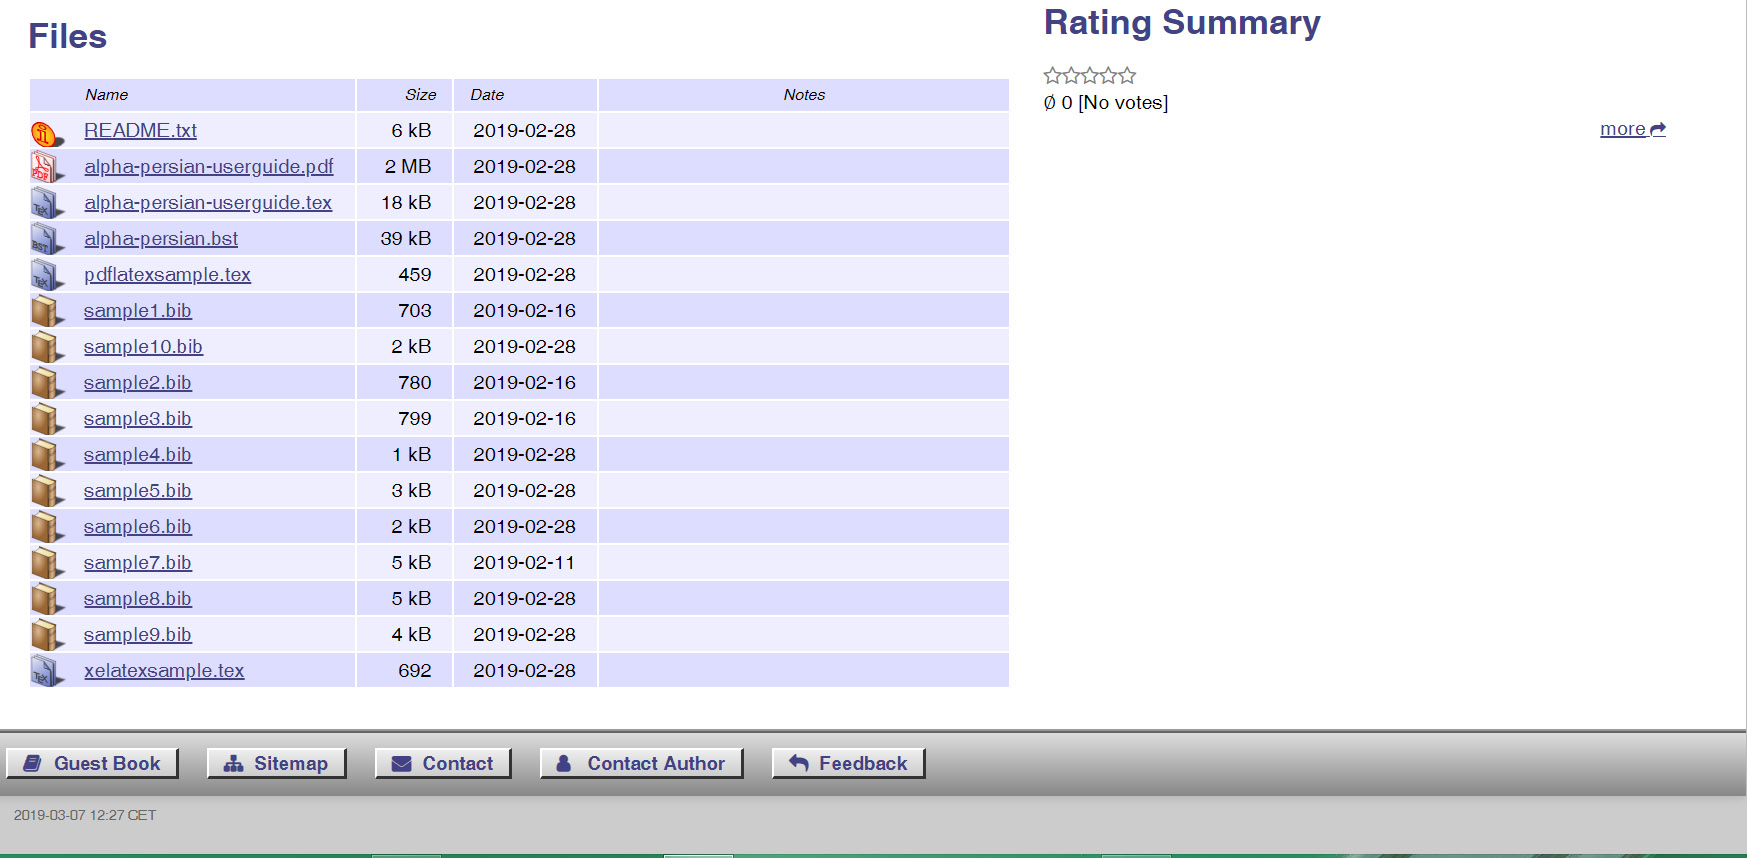
\includegraphics[width=\textwidth,height=8cm]{image/21}
\end{figure}
\section{دیباچه}
پروژه‌ی
\lr{\TeX}
در سال 1978   در  دانشگاه استنفورد توسط 
\textcolor{red}{\textbf{دونالد کنوث}}
شروع شد.  او در ابتدا تخمین زده بود که حدود شش ماه 
این کار را به اتمام می‌رساند اما در نهایت  مراحل انجام این‌کار 
نزدیک به ده سال طول کشید.
یک سال پس از آغاز پروژه‌اش، کنوث به 
یکی از سخنرانی مهم خود در نشست سالانه 
\lr{AMS}
دعوت شد. او درباره‌ی کار خود در 
\lr{\TeX}
از دید نه تنها جنبه‌های تایپی، 
بلکه ایده‌های ریاضی که در پشت برنامه بود،  صحبت  کرد.
در سال 1985،
\linebreak
\textcolor{blue}{\textbf{لزلی لمپورت}}
با معرفی 
\lr{\LaTeX}  
کمک مهمی به  محبوبیت 
\lr{\TeX}
کرد. در واقع
\lr{\LaTeX}
مجموعه‌ای از ماکروها
است که اجازه می‌دهد تا 
نویسندگان به تعامل با سیستم در یک سطح بالاتر از کنوث 
بپردازند. امروزه، سیستم 
\lr{\TeX}
همچنان یک استاندارد شناخته می‌شود. 
حق کپی رایت این نرم افزار بر عهده ی انجمن ریاضی آمریکا
\LTRfootnote{(AMS) American Mathematical Society}
می‌باشد. 
این نرم افزار به صورت رایگان در دسترس قرار دارد. با نرم 
افزار لاتک امروزه می‌توان پایان‌نامه، مقاله‌، کتاب، رزومه، نامه‌ی 
اداری‌، طرح سوال امتحانی و اسلاید به سبک بیمر برای دفاع 
و... تهیه کرد.
\subsection{مزیتها‌ی لاتک در مقایسه با حروف‌چین‌های دیگر}
\begin{enumerate}
\item 
لاتک دارای بهترین خروجی است. خروجی آن معمولاً به صورت پی‌دی‌اف مورد نیاز است که با یک پردازش ساده قابل دسترسی است و
نیازی به نرم‌افزارهای جانبی برای این‌کار ندارد.
\item 
لاتک به خوبی به حروف‌چینی واقف است. فاصله‌ی بین کلمات و حروف استاندارد (و قابل تغییر) بوده و در زمینه‌های چیدن پارگراف‌ها
و ... بی‌نظیر است.
\item 
لاتک سریع است. این بدان معنی است که با یک پردازش ساده 
می‌توانید خروجی مورد نیاز خود در متن یا کارهای گرافیکی و درج تصویر و ... در زمانی مناسب دریافت کنید.
\item 
لاتک ثبات دارد. (با بردن متون لاتک به دستگاه‌های دیگر، 
فرم نوشته‌ها به هم نمی‌ریزد)
\item 
لاتک در عین ثباتش منعطف است. 
رسم جداول و نوشتن مراجع و فراخوانی تصاویر  و ارجاع‌ها و 
.... در آن مشکل نیست.
\item 
ورودی لاتک به صورت متنی است قابل حمل به دستگاه‌های 
دیگر و دارای حجم کم است و برای استایل‌های خاص مانند مقاله،
کتاب و ... به صورت 
پیش‌فرض تنظیمات دارد.
\item 
خروجی آن به فرمتهای 
\lr{HTML}
یا
\lr{PDF}
یا
\lr{PostScript}
قابل تبدیل است.
\item 
قابل اجرا بر روی بیشتر سیستم‌ها از جمله ویندوز و
مکینتاش و .... است (مستقل از سیستم عامل است).
\item 
لاتک بسیار مناسب و استاندارد برای کلیه‌ی مجامع علمی و 
... می‌باشد.
\item
لاتک رایگان است.
\end{enumerate}
\subsection{ایجاد مراجع در لاتک}	
در انتهای هر نوشته، مراجعی که در آن نوشته به آنها ارجاع داده شده
است نوشته می‌شوند. یکی از سبک‌های زیبا و استاندارد جهانی برای
ایجاد مراجع، سبک
\lr{BibTeX}
است. این روش، یک
روش‌ قدرتمند و انعطاف‌پذیر برای نوشتن مراجع مقالات و 
مدیریت مراجع در لاتک است.
	
سبک
\lr{alpha-persian}
که به تازگی توسط این‌جانب تهیه شده است و در 
\href{https://ctan.org/tex-archive/biblio/bibtex/contrib/alpha-persian}{این آدرس}
از 
\lr{CTAN}
قرار گرفته است یکی از سبک‌های
\lr{BibTeX} 
است که 
که برای بسته‌ی زی‌پرشین جهت پشتیبانی از زبان فارسی و همچنین
بدون استفاده از بسته‌ی زی‌پرشن برای نوشته‌های انگلیسی 
 تنظیم شده‌ است. 
\\
قبل از بیان ویژگی‌های این سبک ابتدا جهت آشنایی بهتر با طریقه‌ی
مرجع‌نویسی به کمک 
\lr{BibTeX}،
یک نمونه را در زیر می‌آوریم.
ابتدا یک فایل تک مطابق زیر ایجاد می‌کنیم که در این فایل باید
سبک ظاهر شدن مراجع و همچنین محلی که می‌خواهیم مراجع در
سند ما ظاهر شوند را به صورت زیر در سند خود مشخص کنیم.
\begin{latin}
\begin{Verbatim}[fontsize=\bf,baselinestretch=1,firstnumber=1,formatcom=\color{red!50!black}]
\nocite{*}
\bibliographystyle{alpha-persian}
\bibliography{sample}
\end{Verbatim}
\end{latin}
در دستورات بالا 
\lr{sample}
نام فایلی است با پسوند
\lr{.bib}
که مراجع و موارد مربوط به آنها (نام و نام خانوادگی نویسنده‌ی اثر، 
سال انشار، شابک، شناسه‌ی دیجیتال و ...)
به صورت خام در آنها تعریف می‌شوند.

به عنوان مثال از سبک
\lr{alpha-persian}
در نمونه‌ی بالا استفاده شده است.
توجه کنید که ویژگی‌های ظاهر شدن مراجع و موارد مربوط به آنها در
سبک انتخابی شما تنظیم شده و شما در فایل با پسوند
\lr{.bib}
(در نمونه‌ی بالا منظور همان
\lr{sample.bib}
یا
\lr{sample}
است)
فقط اطلاعات را وارد می‌کنید و تنظیم آنها به طور خودکار و توسط سبک انتخابی شما انجام می‌شود. برای ایجاد فایل 
\lr{bib}
کافی است یک فایل جدید در ویرایشگر خود ایجاد و اطلاعات را در 
آن وارد کنید و سپس در هنگام ذخیره‌ی فایل، پسوند آن را 
\lr{.bib}
(به عنوان نمونه  \lr{sample.bib})
انتخاب کنید و در پوشه‌ی حاوی فایل تک خود قرار دهید. 
دستور
\verb|\nocite{*}|
در دستورات بالا جهت ایجاد مراجع (بدون اینکه به آنها رجوع داده
باشیم) می‌باشد.
\\
این سبک (\lr{alpha-persian}) در مخزن تکلایو و در آدرس زیر قرار دارد:
\begin{latin}
\begin{Verbatim}[fontsize=\bf,baselinestretch=1,firstnumber=1,formatcom=\color{red!50!black}]
Direc­tory biblio/bibtex/contrib/alpha-persian
\end{Verbatim}
\end{latin}
چنان‌چه از تکلایو
2019
به بالا استفاده می‌کنید نیازی به به‌روز کردن آن جهت استفاده از این سبک ندارید. اگر از تکلایو
2018
بهره می‌برید ابتدا مطابق تصاویر زیر تکلایو خود را به روز کنید (در 
مورد توزیع میک‌تک نیز به طور مشابه می‌توان عمل کرد).
\subsection{به‌روز کردن تکلایو}
در قسمت جستجوی ویندوز کلمه‌ی
\lr{tlmgr}
را جستجو کنید و روی آن کلیک کنید تا
\lr{TeX Live Mananger 2018}
مطابق شکل
(\ref{23})
 ظاهر گردد و مراحل انجام کار را مطابق شکل
(\ref{23})
از سر بگیرید. توجه کنید که ممکن است سرعت نت شما قوی نباشد لذا
صبور بوده و مراحل را چند بار انجام دهید تا تکلایو شما به روز شود.
در انتهای تصویر 
(\ref{24})
 گزینه‌ی
\lr{alpha-persian}
 را باید مطابق نمونه تیک زده و گزینه‌ی
\lr{Update}
را تایید کنید.

\begin{figure}[H]
\centering
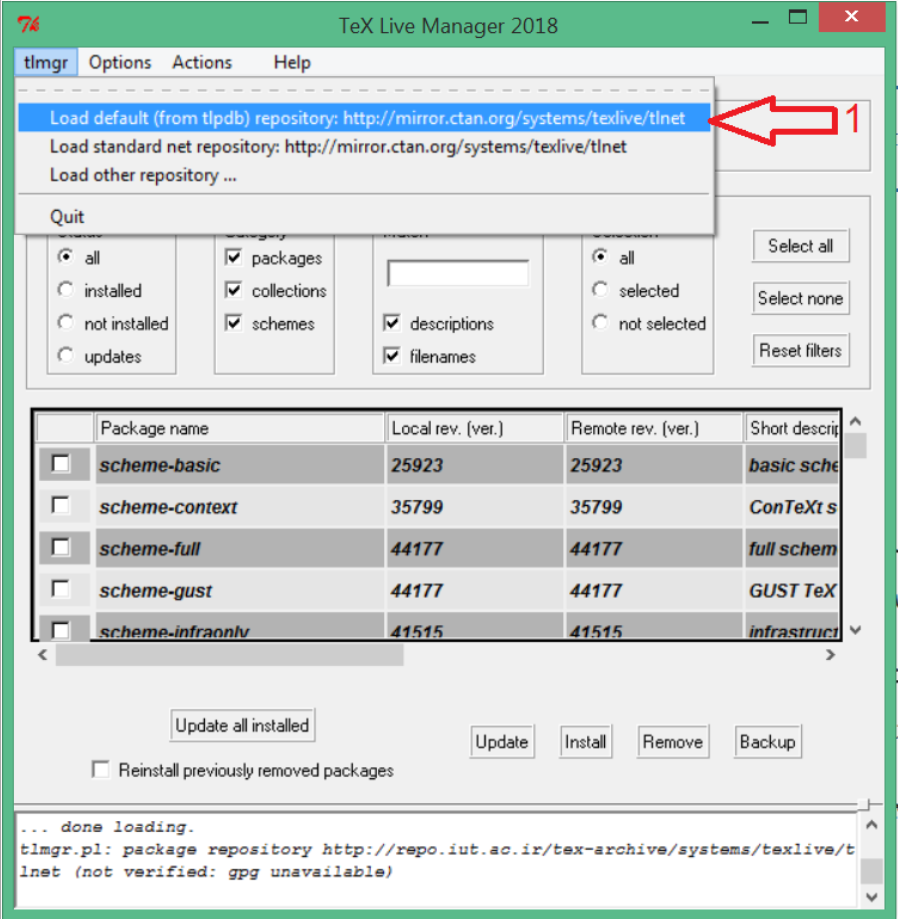
\includegraphics[width=\textwidth,height=14cm]{image/sh14}
\caption{مرحله‌ی اول به‌روز کردن تکلایو}
\label{23}
\end{figure}
\begin{figure}[H]
\centering
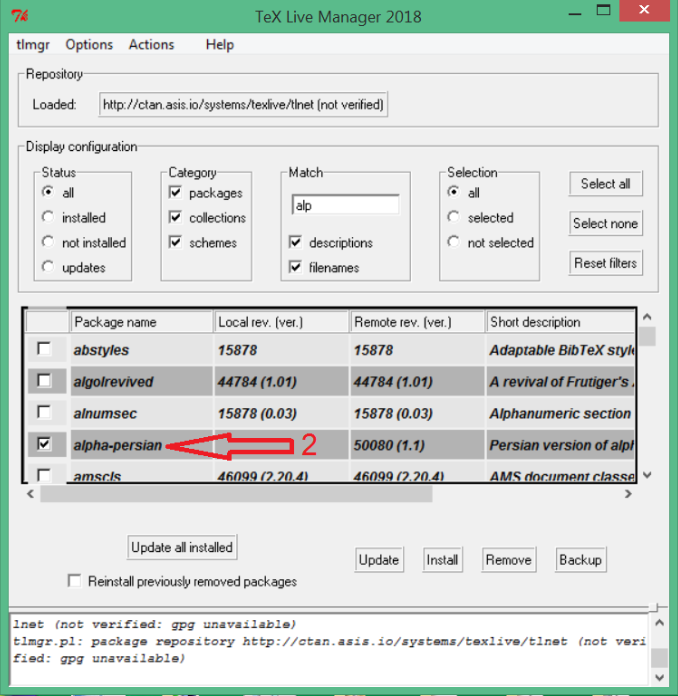
\includegraphics[width=\textwidth,height=16cm]{image/sh15}
\caption{مرحله‌ی دوم به‌روز کردن تکلایو}
\label{24}
\end{figure}
\subsection{یک نمونه‌ی عملی}
\paragraph{نمونه‌ی فایل تک}\hfill
\begin{latin}
\begin{Verbatim}[fontsize=\bf,baselinestretch=1,firstnumber=1,formatcom=\color{red!50!black}]
\documentclass{article}
\usepackage{xcolor}
\usepackage[pagebackref=true,colorlinks,linkcolor=blue,%
citecolor=green!80!black]{hyperref}
\usepackage{xepersian}
\settextfont{Yas}
\begin{document}	
\nocite{*}
\bibliographystyle{alpha-persian}
\bibliography{sample}
\end{document}
\end{Verbatim}
\end{latin}

\paragraph{نمونه‌ی فایل 
\lr{bib}
مطابق نمونه‌ی بالا با نام
\lr{sample.bib}}
این فایل را باید در پوشه‌ی سند خود قرار دهید تا در کنار فایل با 
پسوند
\lr{.tex}
شما باشد و در زمان پردازش مورد استفاده قرار گیرد.
\hfill

\begin{Verbatim}[numbers=left,fontsize=\bf,commandchars=\^\#\*,baselinestretch=1,firstnumber=1,formatcom=\color{green!50!black}]
@article{karamzadeh2012prime,
author={Karamzadeh, Omid Ali Shahny},
title={The Prime Avoidance Lemma Revisited},
key={7},
journal={Kyungpook mathematical journal},
volume={52},
number={2},
pages={149^raisebox#.5mm--* ^!^!^!153},
year={2012},
quotation={1},
publisher={Department of Mathematics, Kyungpook National University}
}
@phdthesis{mmm,
title={^prl#فضای توپولوژی*},
author={^prl# رضایی علی‌آباد,علی*},
journal={Kyungpook mathematical journal},
pages={1163^raisebox#.5mm--* ^!^!^!1171},
LANGUAGE={Persian},
mlabel={^prl#ا.م.ف*},
murl={http://uselatex.com/blog/},
series={second series},
year={2002},
chapter={5},
quotation={1},
school={^prl#دانشگاه چمران اهواز*},
}
\end{Verbatim}
\subsection{پردازش فایل}\label{34}
در مورد پردازش این فایل‌ها بهتر است
(\ref{33})
را ببینید.
\\
می‌توان ویرایش‌‌گر خود را طوری تنظیم کرد که به صورت همزمان نیز
هر چهار مرحله‌ی گفته شده در
(\ref{33})
انجام شود. برای این‌کار ویرایش‌گر خود (تک استودیو)
را باز کنید و از منوی
Options
وارد 
\lr{Configure TeX studio}
شوید و سپس در قسمت
build
یک یوزر جدید مطابق مراحل تصاویر 
(\ref{25})
 ایجاد کنید.
\\
 مطابق شماره‌ها عمل کنید و در مرحله‌ی 4 کدهای زیر را وارد کنید:
\begin{latin}
\begin{Verbatim}[fontsize=\bf,commandchars=\^\#\*,baselinestretch=1,firstnumber=1,formatcom=\color{red!50!black}]
txs:///xelatex |bibtex8 -W -c cp1256fa %.aux| txs:///xelatex|txs:///xelatex
\end{Verbatim}
\end{latin}
\begin{figure}[H]
\centering
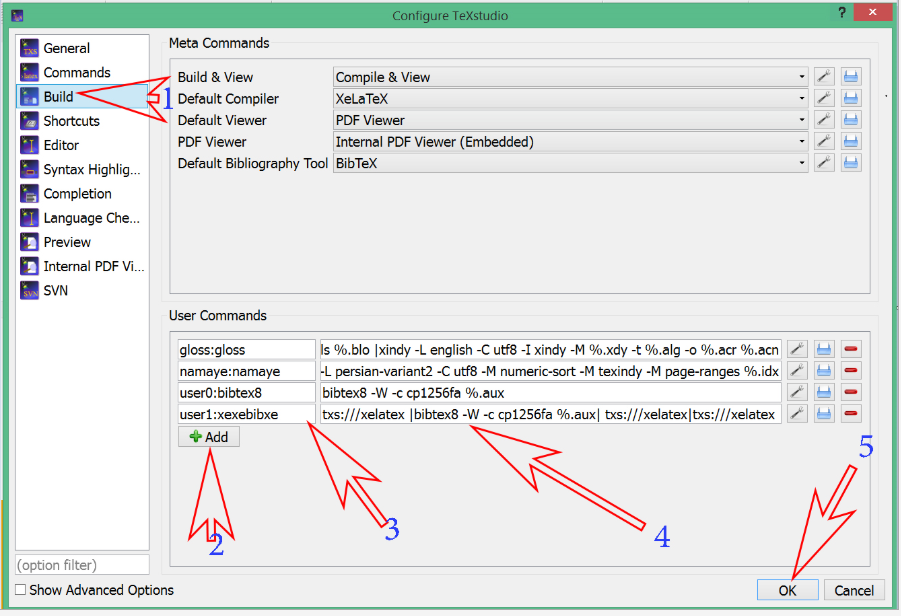
\includegraphics[width=\textwidth,height=10.3cm]{image/sh16}
\caption{مرحله‌ی اول برای ایجاد 
\lr{Command}
جدید}
\label{25}
\end{figure}\vspace*{-.6cm}
\begin{figure}[H]
\centering
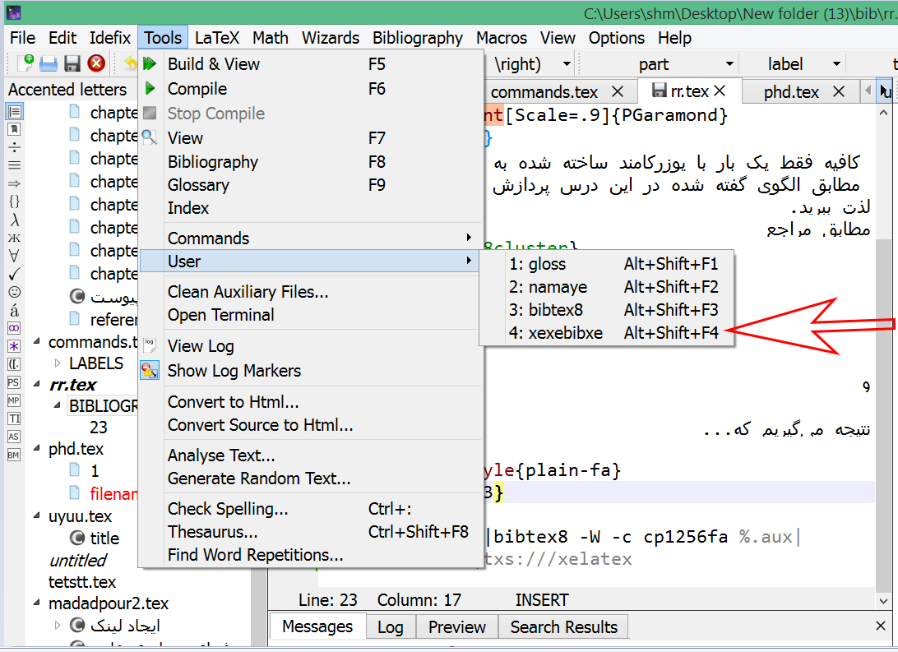
\includegraphics[width=\textwidth,height=9cm]{image/sh17}
\caption{مرحله‌ی دوم برای ایجاد 
\lr{Command}
جدید}
\label{26}
\end{figure}
بعد از انجام 5 مرحله‌ی قبل و تایید مراحل با دکمه‌ی
\lr{ok}
فایل منبع خود را باز کنید و مطابق تصویر
(\ref{26})،
یوزرکامند 
\lr{xexebibxe}
را از منوی
\lr{Tools}
اجرا کنید تا 4 مرحله‌ی پردازش بالا همزمان انجام شوند. \\
با اجرای فرایند فوق
ابتدا مراجع فارسی و سپس لاتین قرار می‌گیرند. 
 در غیر این صورت در مرحله‌ی 4 باید کد‌های زیر را وارد کنید:
\begin{latin}
\begin{Verbatim}[fontsize=\bf,commandchars=\^\#\*,baselinestretch=1,firstnumber=1,formatcom=\color{red!50!black}]
txs:///xelatex |bibtex.exe %| txs:///xelatex|txs:///xelatex
\end{Verbatim}
\end{latin}
بدیهی است که فرایند این مرحله کمی طولانی‌تر از حد معمول است و فقط آن را زمانی انجام دهید که می‌خواهید خروجی نهایی را از فایل خود بگیرید.
\section{%
سبک آلفاپرشین 
با پردازش‌گر زی‌لاتک
\lr{(\XeLaTeX)}}
\label{12}
\noindent
سبک آلفا‌پرشین جهت ایجاد مراجع چپ به راست و راست به چپ تنظیم
گردیده است.

\subsection{طریقه‌ی پردازش فایل در این سبک}\label{33}
زمانی که در سند شما از این سبک استفاده شود به دو طریق 
می‌توانید فایل خود را پردازش کنید.

\paragraph{طریق اول پردازش فایل}
به صورت زیر و با چهار مرحله پردازش
می‌توانید فایل خود را پردازش کنید.
\vspace*{.5cm}
\begin{latin}
{\color{red}$\hookrightarrow$ First Compile:} XeLaTex-BibTeX-XeLaTex-XeLaTex\\
\end{latin}
در این نوع پردازش، ابتدا مراجع با زبان انگلیسی و سپس مراجع با 
زبان فارسی قرار می‌گیرند.
\paragraph{\color{blue} نمونه}

\begin{Verbatim}[numbers=left,fontsize=\bf,commandchars=\^\#\*,baselinestretch=1,firstnumber=1,formatcom=\color{green!50!black}]
@article{karamzadeh2012prime,
author={Karamzadeh, Omid Ali Shahny},
title={The Prime Avoidance Lemma Revisited},
key={7},
journal={Kyungpook mathematical journal},
volume={52},
number={2},
pages={149^raisebox#.5mm--* ^!^!^!153},
year={2012},
quotation={1},
publisher={Department of Mathematics, Kyungpook National University}
}
@phdthesis{mmm,
title={^prl#فضای توپولوژی*},
author={^prl# رضایی علی‌آباد,علی*},
journal={Kyungpook mathematical journal},
pages={1163^raisebox#.5mm--* ^!^!^!1171},
LANGUAGE ={Persian},
mlabel={^prl#ا.م.ف*},
murl={http://uselatex.com/blog/},
series={second series},
year={2002},
chapter={5},
quotation={1},
school={^prl#دانشگاه چمران اهواز*},
}
\end{Verbatim}
\begin{figure}[H]
\centering
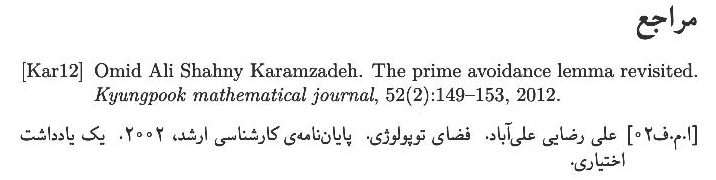
\includegraphics[width=\textwidth,height=3.6cm]{image/sh11}
\end{figure}
\paragraph{طریق دوم پردازش فایل}
به صورت زیر می‌توانید فایل خود را پردازش کنید.
\vspace*{.5cm}
\begin{latin}
{\color{red}$\hookrightarrow$ Second Compile:} XeLaTex-BibTeX 8 bit-XeLaTex-XeLaTex\\
\end{latin}
که در آن منظور از پرازش
{\lr {\tt BibTeX 8 bit}}
ایجاد یک
{\lr {\tt User Command}}
در ویرایش‌گر خود و مطابق با
(\ref{34})
 و با دستور زیر در مرحله‌ی 4 از آن است:
\begin{latin}
\begin{Verbatim}[fontsize=\bf,commandchars=\^\#\*,baselinestretch=1,firstnumber=1,formatcom=\color{red!50!black}]
bibtex8 -W -c cp1256fa %.aux
\end{Verbatim}
\end{latin}
در این نوع پردازش، ابتدا مراجع با زبان فارسی و سپس مراجع با 
زبان انگلیسی قرار می‌گیرند.
\begin{figure}[H]
\centering
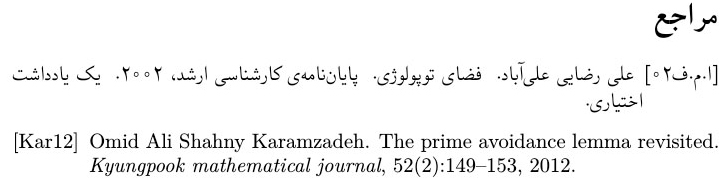
\includegraphics[width=\textwidth,height=3.5cm]{image/sht}
\end{figure}
\subsection{ایجاد کوتیشن‌مارک ("عنوان نوشته``) برای عنوان نوشته به صورت خودکار}
چنان‌چه بخواهید عنوان مقاله‌ی شما به صورت خودکار و به همراه 
کوتیشن‌مارک (علامت نقل قول) ظاهر
گردد کافی است فیلد 
\lr{quotation} 
را در فایل 
\lr{bib}
و به صورت زیر پر کنید:
\begin{latin}
\begin{Verbatim}[fontsize=\bf,commandchars=\^\#\*,baselinestretch=1,firstnumber=1,formatcom=\color{red!50!black}]
quotation={1},
\end{Verbatim}
\end{latin}
\paragraph{\color{blue} نمونه}
نمونه‌‌ی  زیر را ببینید:
\begin{Verbatim}[numbers=left,fontsize=\bf,commandchars=\^\#\*,baselinestretch=1,firstnumber=1,formatcom=\color{green!50!black}]
@article{karamzadeh2012prime,
author={Karamzadeh, Omid Ali Shahny},
title={The Prime Avoidance Lemma Revisited},
key={7},
journal={Kyungpook mathematical journal},
volume={52},
number={2},
pages={149^raisebox#.5mm--* ^!^!^!153},
year={2012},
quotation={1},
madadurltest={1},
murl={http://uselatex.com/blog/},
publisher={Department of Mathematics, Kyungpook National University}
}
@phdthesis{mmm,
title={^prl#فضای توپولوژی*},
author={^prl#رضایی علی‌آباد,علی*},
journal={Kyungpook mathematical journal},
pages={1163^raisebox#.5mm--* ^!^!^!1171},
LANGUAGE={Persian},
mlabel={^prl#ا.م.ف*},
madadurltest={1},
quotation={1},
murl={http://uselatex.com/blog/},
series={second series},
year={2002},
chapter={5},
school={^prl#دانشگاه چمران اهواز*},
}
\end{Verbatim}
\begin{figure}[H]
\centering
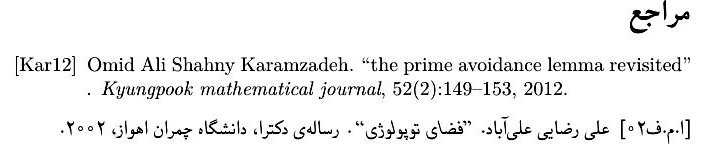
\includegraphics[width=\textwidth,height=3.5cm]{image/sh2}
\end{figure}
\subsection{ایجاد لینک در سبک آلفاپرشین}
 در این سبک به سه طریق می‌توان لینک ایجاد کرد; که یکی از 
 شاخصه‌های منحصر به فرد این سبک است.
\paragraph{طریق اول، ایجاد لینک مخفی برای عنوان:}
در این روش عنوان، به کمک بسته‌ی هایپررف 
\lr{(hyperref)}
به صورت لینک‌دار ظاهر می‌گردد و خود آدرس اینترنتی ظاهر نمی‌گردد. در این روش کافی است دو فیلد زیر را در فایل
\lr{bib}
پر کنید; که در آن محتویات
\lr{murl}
لینک مورد نظر شماست:
\begin{latin}
\begin{Verbatim}[fontsize=\bf,commandchars=\^\#\*,baselinestretch=1,firstnumber=1,formatcom=\color{red!50!black}]
madadurltest={1},
murl={http://uselatex.com/blog/},
\end{Verbatim}
\end{latin}
\paragraph{طریق دوم، ایجاد لینک آشکار}
برای ایجاد این نوع لینک کافی است مطابق زیر و 
\textbf{فقط} 
فیلد 
\lr{url} 
را پرکنید:
\begin{latin}
\begin{Verbatim}[fontsize=\bf,commandchars=\^\#\*,baselinestretch=1,firstnumber=1,formatcom=\color{red!50!black}]
url={http://uselatex.com/blog/},
\end{Verbatim}
\end{latin}
در این حالت خود لینک در مراجع ظاهر می‌گردد و همچنین در حالت 
مراجع فارسی از کلمه‌ی لینک به جای 
\lr{URL}
استفاده می‌شود.
\paragraph{طریق سوم}
ترکیب دو روش بالا نیز مانند زیر امکان‌پذیر است:
\begin{latin}
\begin{Verbatim}[fontsize=\bf,commandchars=\^\#\*,baselinestretch=1,firstnumber=1,formatcom=\color{red!50!black}]
madadurltest={1},
murl={http://uselatex.com/blog/},
url={http://uselatex.com/blog/},
\end{Verbatim}
\end{latin}
نمونه‌‌های
(\ref{112})
را در این زمینه ببینید.
\subsection{پشتیبانی از بسته‌ی هایپررف جهت ایجاد لینک برای عنوان نوشته (لینک مخفی و لینک آشکار)}\label{112}
برای ایجاد لینک‌های مورد نظر کافی است بسته‌ی هایپررف را به صورت
زیر قبل از بسته‌ی زی‌پرشین و در مقدمه‌ی سند فراخوانی کنید.
\begin{latin}\noindent
\begin{Verbatim}[fontsize=\bf,commandchars=\^\#\*,baselinestretch=1,firstnumber=1,formatcom=\color{red!50!black}]
\usepackage[pagebackref=true,colorlinks,linkcolor=blue]{hyperref}
\usepackage{xepersian}
\settextfont{Yas}
\end{Verbatim}
\end{latin}
\paragraph{\color{blue} نمونه}
نمونه‌‌ی ایجاد لینک مخفی برای مقاله را در زیر ببینید:
\begin{figure}[H]
\centering
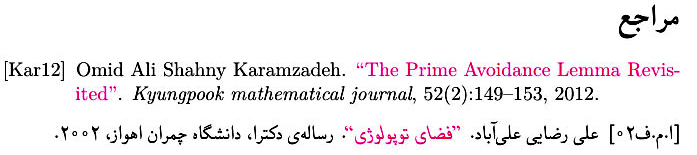
\includegraphics[width=\textwidth,height=3.6cm]{image/sh3}
\end{figure}
\subsection{ایجاد 
\lr{{\large url}}
بدون استفاده از بسته‌های یو‌آر‌اِل و هایپررف}
این قابلیت در این سبک وجود دارد که می‌توان در صورت لزوم و عدم
استفاده از بسته‌های
\lr{url}
و
\lr{hyperref}
فیلد 
\lr{url}
را ایجاد کرد.
\paragraph{\color{blue} نمونه در صورت وجود بسته‌ی 
\lr{hyperref}‌}

\begin{Verbatim}[numbers=left,fontsize=\bf,commandchars=\^\#\*,baselinestretch=1,firstnumber=1,formatcom=\color{green!50!black}]
@article{karamzadeh2012prime,
author={Karamzadeh, Omid Ali Shahny},
title={The Prime Avoidance Lemma Revisited},
key={7},
journal={Kyungpook mathematical journal},
volume={52},
number={2},
pages={149--153},
year={2012},
quotation={1},
url={http://uselatex.com/blog/},
publisher={Department of Mathematics, Kyungpook National University}
}
@phdthesis{mmm,
title={^prl#فضای توپولوژی*},
author={^prl#رضایی علی‌آباد,علی*},
journal={Kyungpook mathematical journal},
pages={1163^raisebox#.5mm--* ^!^!^!1171},
LANGUAGE={Persian},
mlabel={^prl#ا.م.ف*},
madadurltest={1},
quotation={1},
murl={http://uselatex.com/blog/},
series={second series},
year={2002},
url={http://uselatex.com/blog/},
chapter={5},
school={^prl#دانشگاه چمران اهواز*},
}
\end{Verbatim}
\begin{figure}[H]
\centering
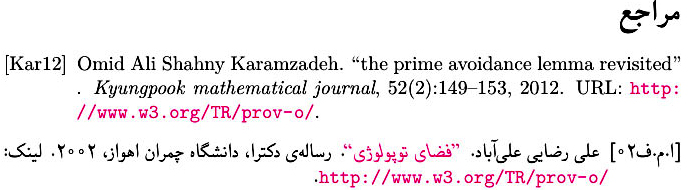
\includegraphics[width=\textwidth,height=4.5cm]{image/sh4}
\end{figure}
\paragraph{\color{blue} نمونه در صورت عدم وجود بسته‌های 
\lr{hyperref}
و
\lr{url}}
نمونه‌ی زیر را در این زمینه ببینید.
\begin{figure}[H]
\centering
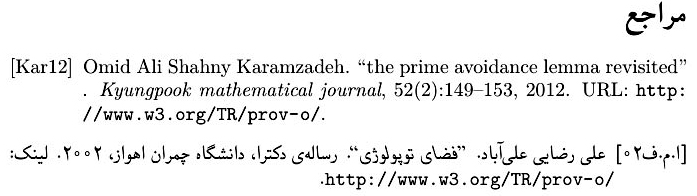
\includegraphics[width=\textwidth,height=4cm]{image/sh5}
\end{figure}
\subsection{ایجاد doi (شناسه‌ی دیجیتال)، isbn (شابک) و issn (شاپا) در یک نوشته}
این سه قابلیت را سبک
\lr{alpha}
 دارا نیست. در سبک
\lr{alpha-persian}
این قابلیت‌ها به آن در حالت لاتین و فارسی افزوده شده است. 
در این سبک 
\lr{(alpha-persian)}
 نام فارسی آنها (شناسه‌ی دیجیتال، شابک و شاپا) 
و به طور خودکار در مراجع فارسی اعمال می‌شود.
\paragraph{\color{blue} نمونه‌ی ورودی در فایل
\lr{bib}}
به صورت زیر می‌توانید اطلاعات را در فایل
\lr{bib}
وارد کنید.
\begin{latin}\noindent
\begin{Verbatim}[fontsize=\bf,commandchars=\^\#\*,baselinestretch=1,firstnumber=1,formatcom=\color{red!50!black}]
issn={1111-2222},
doi={01.1000/doi-0121},
isbn={123456789000},
\end{Verbatim}
\end{latin}
\paragraph{\color{blue} نمونه‌ی کلی در فایل
\lr{bib}}\hfill

\begin{latin}
\begin{Verbatim}[numbers=left,fontsize=\bf,commandchars=\&\#\*,baselinestretch=1,firstnumber=1,formatcom=\color{green!50!black}]
@inbook{d,
AUTHOR={&prl#مددپور, شاپور* and &prl#مددپور, محمدحسین* and &prl#سایرین*},
mlabel={&prl#مدد$^+$*},
TITLE={&prl#همریختی و بروریختی در حلقه‌ها*},
JOURNAL={&prl#مجله‌ی گراف فارس*},
VOLUME ={1},
YEAR={1395},
MONTH={&prl#بهار*},
PAGES={39&raisebox#.5mm--* &!&!&!43},
quotation={1},
LANGUAGE={Persian},
url={http://uselatex.com/blog/},
doi={01.1000/doi-0121},
isbn={123456789000},
edition={&prl#دوم*},
series={&prl#سری دوم*},
number={10},
chapter={5},
madadurltest={1},
murl={http://uselatex.com/blog/},
publisher={&prl#انتشارات دل آهنگ*},
note={&prl#یک یادداشت اختیاری در این‌جا می‌توانید وارد کنید*},
address={&prl#آدرس منتشر کننده*},
}
@book{kuznetsov1998elements,
title={Elements of applied bifurcation theory},
volume={112},
madadurltest={1},
year={1998},
edition={third},
publisher={Springer Verlag},
murl={http://uselatex.com/blog/},
isbn={123456789000},
number={10},
pages={10&raisebox#.5mm--* &!&!&!19},
series={second series},
chapter={5},
issn={1111-2222},
doi={01.1000/doi-0121},
editor={Kuznetsov, Y.A. and edward, Y.A.},
address={The address of the publisher},
}
\end{Verbatim}
\end{latin}
\begin{figure}[H]
\centering
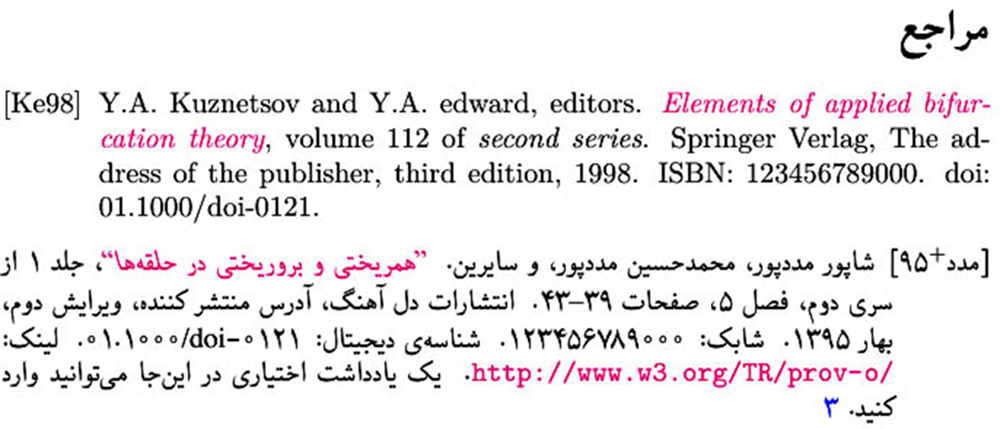
\includegraphics[width=\textwidth,height=6.5cm]{image/sh6}
\end{figure}
\subsection{تنوع برچسب مراجع در سبک آلفاپرشین}
شاید مهمترین ویژگی این سبک، تنوع در برچسب 
\lr{(label)}
 دادن به مراجع است. در سبک
\lr{alpha}
و در حالت پیش‌فرض، مراجع بر اساس نام خانوادگی نویسنده مرتب 
می‌شوند.
\paragraph{حالت اول}
در این سبک با پرکردن فیلد
\lr{slabel}
 و مطابق نمونه‌ی زیر می‌توانید برچسب دلخواه 
 (تعریف شده در لاتک) برای مراجع خود انتخاب کنید:
\begin{Verbatim}[numbers=left,fontsize=\bf,commandchars=\&\#\*,baselinestretch=1,firstnumber=1,formatcom=\color{green!50!black}]
slabel={$\checkmark\checkmark\checkmark$},
OR
slabel={$\spadesuit$},
OR
slabel={$\clubsuit$},
\end{Verbatim}
\begin{figure}[H]
\centering
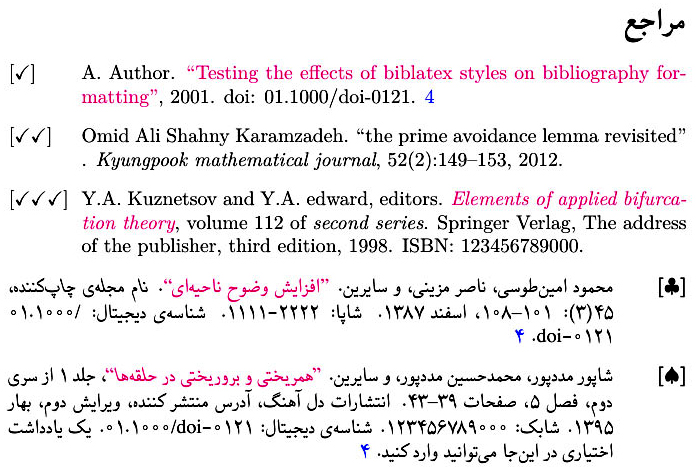
\includegraphics[width=\textwidth,height=11cm]{image/sh7}
\end{figure}
این ویژگی منحصر به فرد
برجسب‌گذاری برای برچسب‌ها این اختیار را به ما می‌دهد 
که از سیستم شماره‌گذاری عددی نیز به سادگی استفاده کنیم. 
برای انجام این کار ابتدا پردازش کنید و سپس با توجه به ترتیب سبک 
\lr{alpha}
 شماره‌ی مراجع را انتخاب کنید که بر حسب نام خانوادگی نویسنده است. در ادامه و در
(\ref{32})
 می‌بینیم که می‌توان مراجع را با ترتیب دلخواه نیز مرتب کرد.
نمونه‌‌ی زیر را ببینید.
\begin{latin}
\begin{Verbatim}[numbers=left,fontsize=\bf,commandchars=\&\#\*,baselinestretch=1,firstnumber=1,formatcom=\color{green!50!black}]
slabel={1},
OR
slabel={2},
OR
slabel={3},
OR
slabel={4},
\end{Verbatim}
\end{latin}
\begin{figure}[H]
\centering
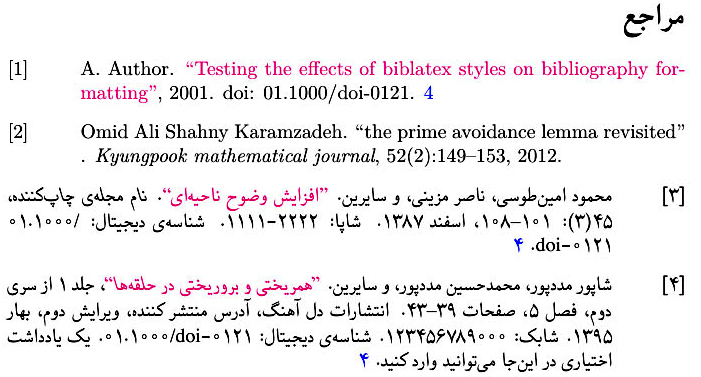
\includegraphics[width=\textwidth,height=8cm]{image/sh8}
\end{figure}
\paragraph{حالت دوم}
نوع دیگر ایجاد بر چسب، استفاده از حالت پیش‌فرض سبک 
\lr{alpha} 
است. در ای حالت برای مراجع لاتین نیازی به پرکردن فیلدی برای برچسب نیست اما به دلیل متفاوت بودن ساختار زبان فارسی و انگلیسی برای مراجع فارسی باید از فیلد 
\lr{mlabel}
کمک و یکی از دو حالت زیر استفاده کنید.
\begin{itemize}
\item 
چنان‌چه فقط یک نویسنده داشته باشید سه حرف اول از بخش
 آخر نام خانوادگی نویسنده (با یا بدون یک جداکننده‌ی دلخواه بین 
 حروف) را انتخاب کنید; به عنوان نمونه اگر نویسنده‌ی مقاله علی 
رضایی علی‌آباد باشد به صورت زیر فیلد 
\lr{mlabel} 
را پر کنید (یا روش دلخواه دیگر):
\begin{latin}
\begin{Verbatim}[fontsize=\bf,commandchars=\&\#\*,baselinestretch=1,formatcom=\color{red!50!black}]
mlabel ={&prl#ع.ل.ی*}
\end{Verbatim}
\end{latin}
\item 
اگر چند نویسنده داشته باشید حروف اول از ابتدای بخش آخر نام 
خانوادگی (با یا بدون یک جداکننده‌ی دلخواه بین حروف)
نویسندگان را انتخاب 
کنید; به عنوان نمونه اگر نویسندگان یک مقاله به ترتیب وفا خلیفی، 
وحید دامن‌افشان و سید جواد رضویان باشند به صورت زیر فیلد 
\lr{mlabel}
را پر کنید (یا روش دلخواه دیگر):
\begin{latin}
\begin{Verbatim}[fontsize=\bf,commandchars=\&\#\*,baselinestretch=1,formatcom=\color{red!50!black}]
mlabel ={&prl#خ.د.ر*}
\end{Verbatim}
\end{latin}
\end{itemize}
\paragraph{نکته‌ی مهم}
معمولاً زمانی که تعداد نویسندگان یک نوشته بیشتر از سه نفر باشند 
تمایل بر این است که در مراجع لاتین از عبارت
\lr{«et all»}
 و در فارسی از کلمه‌ی «سایرین» در نوشتن مراجع استفاده شود.
برای ایجاد این نوع مراجع به صورت زیر عمل کنید:
\\
چنان‌چه در مراجع لاتین بخواهیم این اتفاق رخ دهد کافی است در انتهای نوشتن آن مرجع عبارت
\lr{«and others»}
 را به صورت زیر وارد کنید:
\begin{latin}
\begin{Verbatim}[fontsize=\bf,commandchars=\&\#\*,baselinestretch=1,formatcom=\color{red!50!black}]
author={Rezaei, Ali and Namdari, Mehrdad and Eatemadi, Ali. and others},
\end{Verbatim}
\end{latin}
در این حالت در برچسب این مرجع به طور خودکار بین نام و سال 
نوشته‌شدن آن نوشته یک «+» و در حالت توان و به زیبایی ایجاد 
می‌شود.
چنان‌چه در مراجع فارسی بخواهیم این اتفاق رخ دهد کافی است 
در انتهای نوشتن آن مرجع به صورت زیر عمل کنید:
\begin{latin}
\begin{Verbatim}[fontsize=\bf,commandchars=\&\#\*,baselinestretch=1,formatcom=\color{red!50!black}]
author={&prl#امین‌طوسی,محمود* and&prl# مزینی ,ناصر* and &prl#سایرین*},
\end{Verbatim}
\end{latin}
در این حالت باید در
\lr{mlabel}
به صورت زیر 
\verb|$^+$|
را ایجاد کنید:
\begin{latin}
\begin{Verbatim}[fontsize=\bf,commandchars=\&\#\*,baselinestretch=1,formatcom=\color{red!50!black}]
mlabel = {&prl#ا.م*$^+$},
\end{Verbatim}
\end{latin}
نمونه‌ی
(\ref{35})
را ببنید.
\subsection{سازگاری این سبک با بسته‌های
\lr{{\large cite}}
و
\lr{{\large natbib}}}\label{35}
این سبک اگر با بسته‌های فوق به کار رود ایجاد مشکل نخواهد کرد.
برای فشرده کردن ارجاعات متوالی معمولاً به همراه این سبک
از این بسته‌ها کمک می‌گیریم.

\begin{latin}
\begin{Verbatim}[fontsize=\bf,commandchars=\^\#\*,baselinestretch=1,firstnumber=1,formatcom=\color{red!50!black}]
\usepackage[numbers,sort&compress]{natbib}
\usepackage[compress]{cite} 
\end{Verbatim}
\end{latin}\vspace*{-.8cm}
\paragraph{\color{blue} نمونه}
در نمونه‌ی زیر از بسته‌ی 
\lr{{\large cite}}
برای فشرده‌ کردن ارجاعات متوالی استفاده شده است.
\begin{figure}[H]
\centering
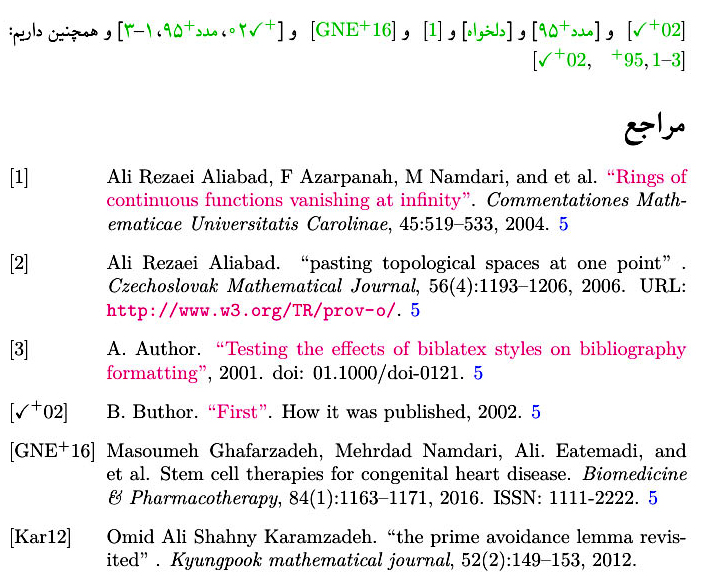
\includegraphics[width=\textwidth,height=12.5cm]{image/sh9}
\end{figure}
\subsection{ترتیب دلخواه برای مراجع}\label{32}
در این سبک می‌توانید به کمک ساختار دستور
\verb|\noopsort| 
مراجع فارسی را با هم و یا مراجع انگلیسی 
را نیز با هم و همچنین هر دو را به صورت ترکیبی بچینیم. 
برای انجام این کار ماکروی 
\verb|\noopsort|
برای این سبک تنظیم شده است که می‌توانید آن را برای نام خانوادگی نویسنده‌ و به صورت زیر به کار ببرید:
\begin{latin}
\begin{Verbatim}[fontsize=\bf,commandchars=\^\#\*,baselinestretch=1,firstnumber=1,formatcom=\color{red!50!black}]
AUTHOR = "{\noopsort{1}}{Madadpour},Shapour  ",
\end{Verbatim}
\end{latin}
توجه کنید چنان‌چه بخواهید تمام مراجع را به صورت دستی 
مرتب کنید باید برای تمام مراجع این‌کار را انجام دهید.
\\
پردازش این‌گونه فایل‌ها باید به صورت 
زیر برای زی‌لاتک و یا پی‌دی‌اف لاتک انجام شود:
\begin{latin}
\begin{Verbatim}[fontsize=\bf,commandchars=\^\#\*,baselinestretch=1,firstnumber=1,formatcom=\color{red!50!black}]
XeLaTex-BibTeX-XeLaTex-XeLaTex
OR
pdfLaTeX-BibTeX-pdfLaTeX-pdfLaTeX
\end{Verbatim}
\end{latin}
\begin{Verbatim}[numbers=left,fontsize=\bf,commandchars=\&\#\*,baselinestretch=1,firstnumber=1,formatcom=\color{green!50!black}]
@misc{whatever,
AUTHOR="{\noopsort{2}}{Madadpour},Ahmad ",
quotation={1},
year={2001},
chapter={5},
title={Testing the effects of bibtex styles on bibliography formatting},
murl={http://www.w3.org/TR/prov-o/},
doi={01.1000/doi-0121},
madadurltest={1},
key={665},
}
@misc{B02f,
howpublished={How it was published},
AUTHOR="{\noopsort{4}}{Madadpour},Shapour  ",
year={2002},
quotation={1},
title={First},
pages={13&raisebox#.5mm--* &!&!&!17},
madadurltest={1},
mlabel={$\checkmark^+$},
murl={http://www.w3.org/TR/prov-o/},
chapter={5},
}
@article{aliabad2004rings,
title={reference test-Rings of continuous functions vanishing at infinity},
AUTHOR= "{\noopsort{6}}{Madadpour},Alireza ",
journal={Commentationes Mathematicae Universitatis Carolinae},
volume={45},
pages={519&raisebox#.5mm--* &!&!&!533},
quotation={1},
year={2004},
murl={http://www.w3.org/TR/prov-o/},
madadurltest={1},
publisher={Charles University in Prague, Faculty of Mathematics and Physics},
}
@article{ali,
title={reference test-Pasting topological spaces at one point},
AUTHOR= "{\noopsort{8}}{Madadpour},Mahmood ",
journal={Czechoslovak Mathematical Journal},
volume={56},
number={4},
pages={1193&raisebox#.5mm--* &!&!&!1206},
quotation={1},
year={2006},
publisher={Springer},
url={http://www.w3.org/TR/prov-o/},
}
@article{Amintoosi87afzayesh,
TITLE={&prl#افزایش وضوح ناحیه‌ای*},
BOOKTITLE={&prl#چهاردهمین کنفرانس ملی سالانه انجمن کامپیوتر ایران*},
author={{\noopsort{1}}{&prl#امین‌طوسی*}&prl#محمود, * and &prl# مزینی ,ناصر*and &prl#سایرین*},
YEAR ={1387},
ORGANIZATION={&prl#دانشگاه امیرکبیر*},
ADDRESS={&prl#تهران، ایران*},
journal={&prl#نام مجله‌ی چاپ‌کننده*},
month={&prl#اسفند*},
doi={01.1000/doi-0121},
edition={&prl#ششم*},
volume={45},
number={3},
pages={101&raisebox#.5mm--* &!&!&!108},
issn={1111&raisebox#.5mm-* &!&!&!2222},
madadurltest={1},
chapter={5},
quotation={1},
LANGUAGE={Persian},
mlabel={ا.م$^+$},
slabel={$\heartsuit$},
murl={http://www.w3.org/TR/prov-o/},
}
@inbook{d,
AUTHOR={{\noopsort{1}}{&prl#مددپور*}&prl#شاپور, * and &prl# مددپور ,محمدحسین*and &prl#سایرین*},
mlabel={&prl#مدد$^+$*},
TITLE={&prl#همریختی و بروریختی در حلقه‌ها*},
JOURNAL={&prl#مجله‌ی گراف فارس*},
VOLUME={1},
YEAR={1395},
MONTH={&prl#بهار*},
PAGES={39&raisebox#.5mm--* &!&!&!43},
quotation={1},
LANGUAGE={Persian},
doi={&prl#01.1000/doi*&raisebox#.5mm-* &!&!&!0121},
isbn={123456789000},
edition={&prl#دوم*},
series={&prl#سری دوم*},
number={10},
chapter={5},
madadurltest={1},
murl={http://www.w3.org/TR/prov-o/},
publisher={&prl#انتشارات دل آهنگ*},
note={&prl#یک یادداشت اختیاری در این‌جا می‌توانید وارد کنید*},
address={‌&prl#آدرس منتشر کننده*},
slabel={$\bigstar$},
}
@phdthesis{mmm,
title={&prl#فضای توپولوژی*},
author={{\noopsort{5}}{&prl#رضایی علی‌آباد*}&prl#علی,*},
journal={Kyungpook mathematical journal},
pages={1163&raisebox#.5mm--* &!&!&!1171},
LANGUAGE ={Persian},
mlabel={&prl#ا.م.ف*},
madadurltest={1},
quotation={1},
murl={http://www.w3.org/TR/prov-o/},
series={second series},
year={2002},
url={http://www.w3.org/TR/prov-o/},
chapter={5},
school={&prl#دانشگاه چمران اهواز*},
}
@inbook{yu,
author={{\noopsort{1}}{&prl#نامداری*}&prl#مهرداد, * and &prl# کوچک‌پور ,عبدعلی*},
mlabel ={&prl#ن.ا.م$^+$*},
TITLE ={&prl#مقدمه‌ای بر نظریه‌ی  اصولی مجموعه‌ها*},
VOLUME={1},
YEAR={1394},
MONTH={&prl#بهار*},
PAGES={39&raisebox#.5mm--* &!&!&!43},
quotation={1},
LANGUAGE={Persian},
doi={322/511},
isbn={978&raisebox#.5mm-* &!&!&!600&raisebox#.5mm-* &!&!&!141&raisebox#.5mm-* &!&!&!173&raisebox#.5mm-* &!&!&!1},
edition={&prl#دوم*},
series={&prl#سری دوم*},
number={100},
chapter={5},
madadurltest={1},
murl={http://www.w3.org/TR/prov-o/},
publisher={&prl#انتشارات دانشگاه چمران*},
note={&prl#یک یادداشت اختیاری در این‌جا می‌توانید وارد کنید*},
address={&prl#آدرس منتشر کننده*},
slabel={4},
}
\end{Verbatim}
\begin{figure}[H]
\centering
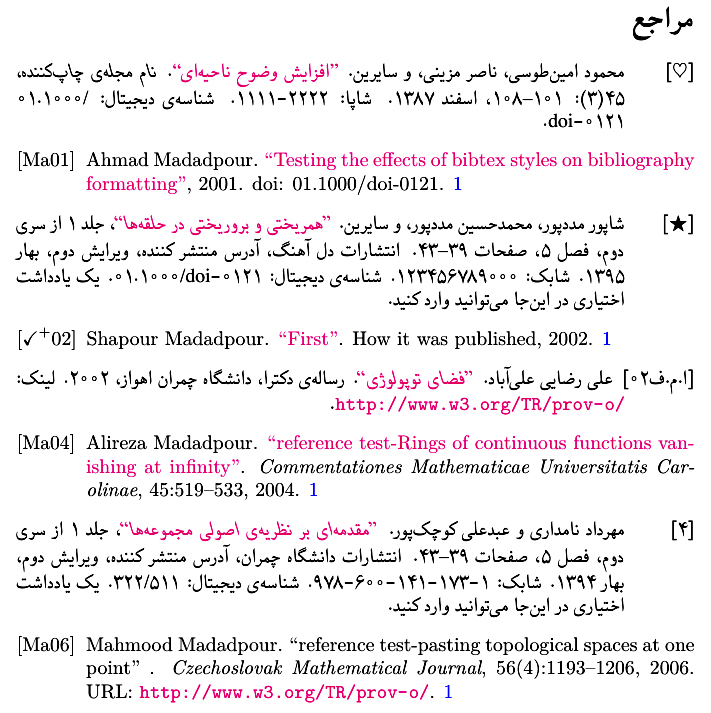
\includegraphics[width=\textwidth,height=15.5cm]{image/sh12}
\end{figure}


\paragraph{یک نمونه‌ی کلی}
فایل
\lr{bib}
این نمونه در
\href{https://ctan.org/tex-archive/biblio/bibtex/contrib/alpha-persian}{این آدرس از 
\lr{CTAN}}
و با نام
\lr{sample8}
قابل دسترسی است.
\\
\noindent
\begin{latin}
{\color{blue}$\hookrightarrow$ Compile: XeLaTex-BibTeX 8 bit-XeLaTex-XeLaTex}\\
\end{latin}
\lr{\cite{B02f}}
 و
\cite{d}
و
\cite{Amintoosi87afzayesh}
و
\lr{\cite{aliabad2004rings}}
و
\lr{\cite{ghafarzadeh2016stem}}
و
\cite{aliabad2004rings,ali,whatever,B02f,d}
و همچنین داریم:
\\
\lr{\cite{aliabad2004rings,ali,whatever,B02f,d}}

\nocite{*}                  
\bibliographystyle{alpha-persian}
%\bibliography{sample1}
%\bibliography{sample2}
%\bibliography{sample3}
%\bibliography{sample4}
%\bibliography{sample5}
%\bibliography{sample6}
%\bibliography{sample7}
\bibliography{sample8}
\newpage
\section{%
سبک آلفاپرشین 
با پردازش‌گر پی‌دی‌اف ‌لاتک
\lr{(\protect \pdflatex)}}
استفاده از سبک آلفاپرشین
بدون بسته‌ی زی‌پرشین و پردازشگر 
\lr{pdfLaTeX}
نیز به سادگی امکان‌پذیر است.
\\
اگرچه این سبک برای استفاده‌ی فارسی‌زبانان و به کمک بسته‌ی 
زی‌پرشین تدارک دیده شده است; اما با قرار دادن ساختار زیرقبل از 
\verb|\begin{document}|
در سند خود می‌توانید با پردازش‌گر 
\lr{pdfLaTeX}
نیز برای اسناد لاتین بهره بگیرید:
\begin{latin}
\begin{Verbatim}[fontsize=\bf,commandchars=\^\#\*,baselinestretch=1,firstnumber=1,formatcom=\color{red!50!black}]
\let\lr\relax  
\let\setlatin\relax
\let\resetlatinfont\relax
\newenvironment{LTRbibitems}{}{}
\end{Verbatim}
\end{latin}
\paragraph{\color{blue} نمونه‌:}\hfill

\begin{latin}
{\color{blue}$\hookrightarrow$ Compile: pdfLaTeX-BibTeX-pdfLaTeX-pdfLaTeX}
\begin{Verbatim}[numbers=left,fontsize=\bf,commandchars=\&\#\*,baselinestretch=1,firstnumber=1,formatcom=\color{green!50!black}]
@misc{whatever,
AUTHOR= "{\noopsort{1}}{Madadpour},Ahmad ",
quotation={1},
year={2001},
chapter={5},
title={Testing the effects of bibtex styles on
bibliography formatting},
murl={http://www.w3.org/TR/prov-o/},
doi={01.1000/doi-0121},
madadurltest={1},
key={665},
}
@misc{B02f,
howpublished = {How it was published},
AUTHOR= "{\noopsort{2}}{Madadpour},Shapour and
Madadpour , Mohamadhosain and Madadpour , Mitra  ",
year={2002},
quotation={1},
title={First},
pages={13--17},
madadurltest={1},
mlabel={&prl#$\checkmark^+$*},
murl={http://www.w3.org/TR/prov-o/},
chapter={5},
}
@article{aliabad2004rings,
title={reference test-Rings of continuous functions
vanishing at infinity},
AUTHOR= "{\noopsort{3}}{Madadpour},Alireza ",
journal={Commentationes Mathematicae Universitatis Carolinae},
volume={45},
pages={519--533},
quotation={1},
year={2004},
murl={http://www.w3.org/TR/prov-o/},
madadurltest={1},
publisher={Charles University in Prague, Faculty of
Mathematics and Physics},
}
@article{ali,
title={reference test-Pasting topological spaces at one point},
AUTHOR = "{\noopsort{4}}{Madadpour},Mahmood ",
journal={Czechoslovak Mathematical Journal},
volume={56},
number={4},
pages={1193--1206},
quotation={1},
year={2006},
publisher={Springer},
url={http://www.w3.org/TR/prov-o/},
}
@book{kuznetsov1998elements,
title={reference test-Elements of
applied bifurcation theory},
volume={112},
madadurltest={1},
year={1998},
edition={third},
publisher={Springer Verlag},
murl={http://www.w3.org/TR/prov-o/},
isbn={123456789000},
number={10},
pages={10--19},
series={second series},
chapter={5},
AUTHOR= "{\noopsort{5}}{Madadpour},Behrooz ",
address={The address of the publisher},
}
\end{Verbatim}
\begin{latin}
{\color{blue}$\hookrightarrow$ Compile: pdfLaTeX-BibTeX-pdfLaTeX-pdfLaTeX}
\end{latin}
\begin{figure}[H]
\centering
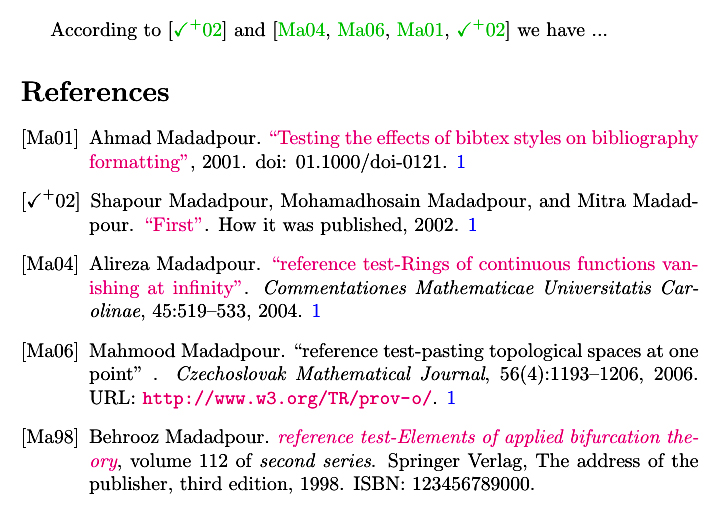
\includegraphics[width=\textwidth,height=11cm]{image/sh13}
\end{figure}
\end{latin}
\paragraph{توجه}
زمانی که از پردازش‌گر پی‌دی‌اف لاتک در اسناد لاتین استفاده می‌کنید 
تمام ویژگیهای پردازش با زی‌لاتک را نیز دارید.


\noindent
برگ سبزیست تحفه‌ی درویش و در پایان امیدوارم مفید واقع 
شود و مجدداً از تمام عزیزان کاربر و صاحب‌نظر خواهشمندم 
با توجه به این‌که تاکنون در گیت‌لب فایل این سبک را قرار 
نداده‌ام، هرگونه پیشنهاد را به ایمیل شخصی این‌جانب در نشانی 
\verb|madad_sh@yahoo.com| 
ارسال کنند و پیشاپیش از همکاری شما عزیزان سپاس‌گزارم. 
درود بر شما.
\begin{center}
{\LARGE نوزدهم اسفند هزار و سیصد و نود و هفت; شاپور مددپور}
\end{center}


\end{document}
